% !TeX root = ../thuthesis-example.tex
\chapter{bolt.SE 系统架构与技术创新}

本章将详细介绍bolt.SE系统的整体架构、核心技术及创新点。bolt.SE基于开源项目bolt.diy构建,保留其核心优势的同时,引入多项技术创新以增强软件工程实践支持。本章首先介绍bolt.diy的基础架构与技术特点,随后重点阐述bolt.SE的创新模块及其在软件工程流程中的应用价值。

\section{bolt.diy介绍}

本项目基于开源项目bolt.diy,在此基础上进行了多方面的优化和扩展。选择bolt.diy作为基础平台的原因主要体现在以下几个方面:

\begin{itemize}
    \item 开源与扩展性: bolt.diy作为开源平台,具备高度扩展性和灵活性,便于根据项目需求进行定制化开发,适应各种软件工程实践要求。
    \item 多种大语言模型支持: bolt.diy支持多种大语言模型(LLM),如GPT-o3-mini、Claude 3.7 Sonnet等,并持续扩展对新模型的支持。
    \item 代码生成能力: bolt.diy能够理解和感知大规模复杂软件项目的上下文信息,在解析代码库和管理项目结构方面表现出色。
    \item WebContainer技术: bolt.diy使用WebContainer技术,使代码能在浏览器中实时执行并预览,提升了开发的交互性和实时响应能力,便于开发者快速验证代码效果。
\end{itemize}

\subsection{系统架构}

bolt.diy系统的工作流程涉及多个核心组件的协同运作,如图~\ref{fig:bolt_sequence}灰色部分所示。整体流程包括以下几个关键步骤:
\begin{enumerate}
    \item 用户通过UI界面输入需求,选择适当的大语言模型(LLM)。
    \item LLM生成自然语言响应,经过MessageParser模块解析为结构化XML格式。
    \item 生成的代码通过FileStore存储,并通过ActionRunner在WebContainer环境中执行。
    \item 执行结果通过ActionRunner反馈给用户,完成代码生成和执行过程。
\end{enumerate}

其中,ActionRunner、FileStore和WebContainer进行交互,WebContainer提供隔离、安全的运行环境,允许代码在浏览器中直接执行。

另外,由于所有代码生成过程本质上都表现为用户与大语言模型之间的交互对话,因此,整个项目的代码库实际上是一系列高度结构化的"对话记录"。利用LLM的长文本处理能力,bolt.diy能够将这些累积的对话历史完整地纳入模型的记忆上下文。这种设计使LLM不仅能基于当前用户输入生成代码,还能回顾并记忆历史生成的代码片段、开发者的设计决策以及代码库整体的架构约定。

\begin{figure}[htbp]
  \makebox[\textwidth][c]{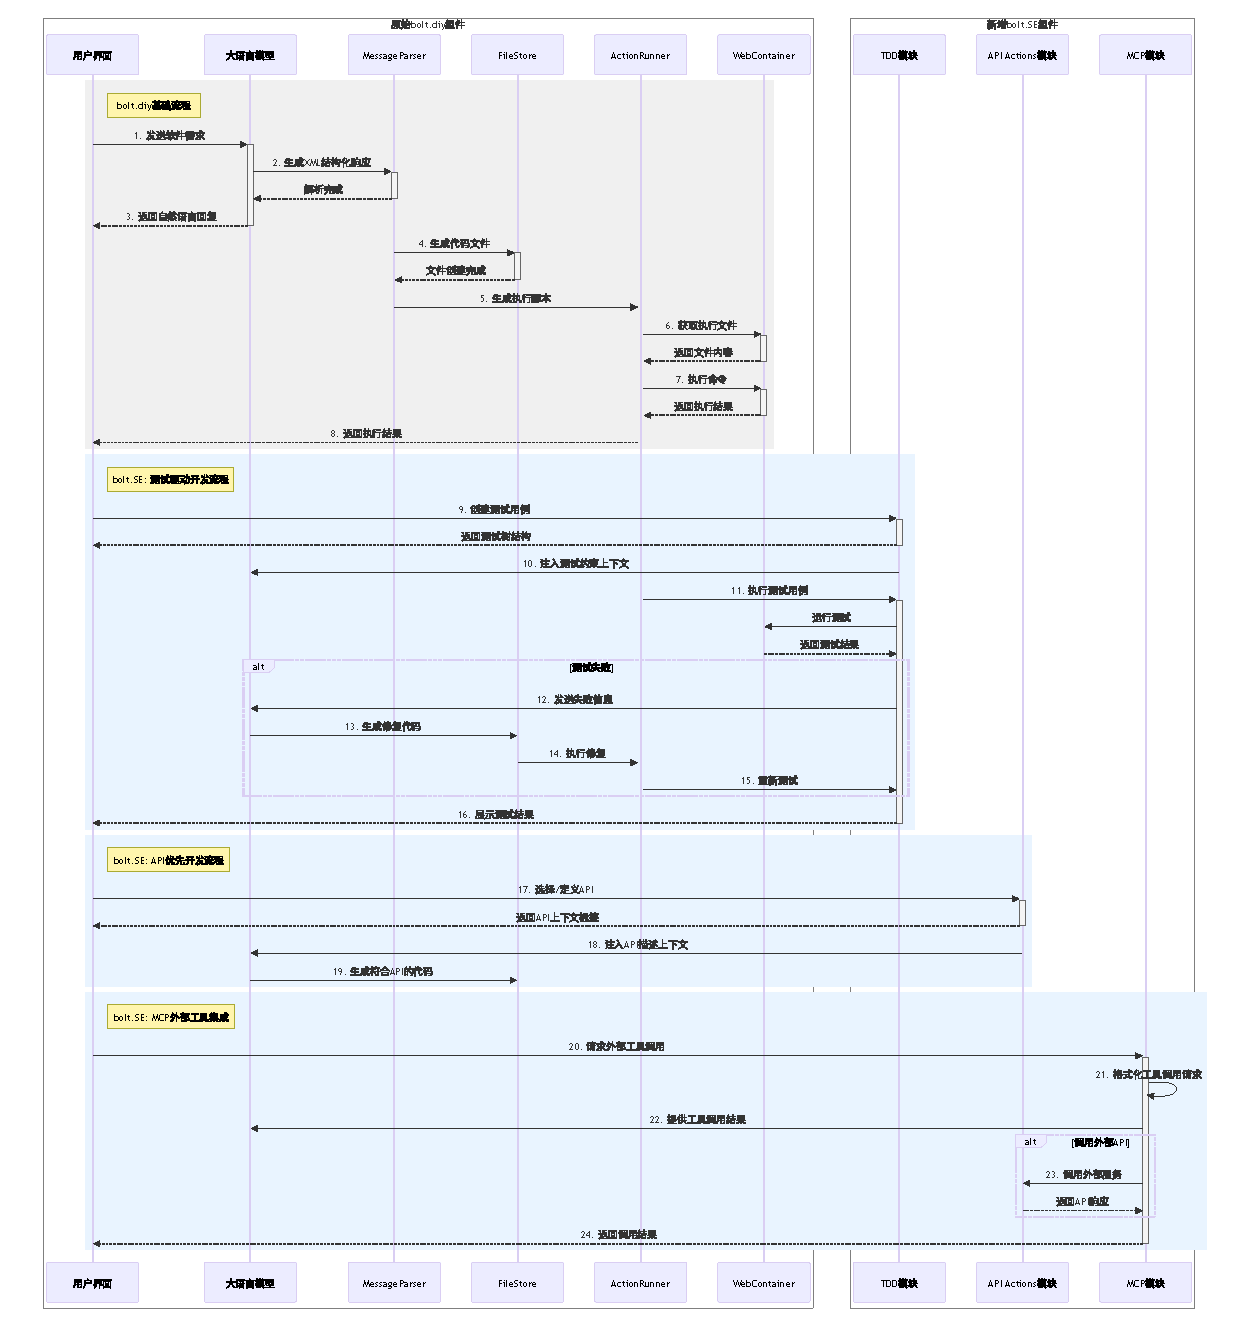
\includegraphics[width=1.3\textwidth]{figures/bolt_sequence.pdf}}
  \caption{bolt.SE系统架构图:显示bolt.diy基础流程(灰色区域)与bolt.SE创新模块(蓝色区域)的集成与交互}
  \label{fig:bolt_sequence}
\end{figure}
% sequenceDiagram
%     %% 使用不同颜色区分bolt.diy和bolt.SE的组件
%     %% bolt.diy组件使用默认颜色,bolt.SE组件使用蓝色
    
%     %% 定义参与者和分组
%     box 原始bolt.diy组件
%     participant UI as 用户界面
%     participant LLM as 大语言模型
%     participant MP as MessageParser
%     participant FS as FileStore
%     participant AR as ActionRunner
%     participant WC as WebContainer
%     end
    
%     box 新增bolt.SE组件
%     participant TDD as TDD模块
%     participant API as API Actions模块
%     participant MCP as MCP模块
%     end
    
%     %% 标注整体流程区域
%     rect rgb(240, 240, 240)
%     note right of UI: bolt.diy基础流程
    
%     %% bolt.diy的标准流程
%     UI->>+LLM: 1. 发送软件需求
%     LLM->>+MP: 2. 生成XML结构化响应
%     MP-->>-LLM: 解析完成
%     LLM-->>-UI: 3. 返回自然语言回复
    
%     MP->>+FS: 4. 生成代码文件
%     FS-->>-MP: 文件创建完成
    
%     MP->>+AR: 5. 生成执行脚本
%     AR->>+WC: 6. 获取执行文件
%     WC-->>-AR: 返回文件内容
    
%     AR->>+WC: 7. 执行命令
%     WC-->>-AR: 返回执行结果
%     AR-->>UI: 8. 返回执行结果
%     end
    
%     %% bolt.SE扩展功能 - 测试驱动开发
%     rect rgb(233, 244, 255)
%     note right of UI: bolt.SE: 测试驱动开发流程
    
%     UI->>+TDD: 9. 创建测试用例
%     TDD-->>-UI: 返回测试树结构
    
%     TDD->>LLM: 10. 注入测试约束上下文
    
%     AR->>+TDD: 11. 执行测试用例
%     TDD->>WC: 运行测试
%     WC-->>TDD: 返回测试结果
    
%     alt 测试失败
%         TDD->>LLM: 12. 发送失败信息
%         LLM->>FS: 13. 生成修复代码
%         FS->>AR: 14. 执行修复
%         AR->>TDD: 15. 重新测试
%     end
    
%     TDD-->>-UI: 16. 展示测试结果
%     end
    
%     %% bolt.SE扩展功能 - API优先开发
%     rect rgb(233, 244, 255)
%     note right of UI: bolt.SE: API优先开发流程
    
%     UI->>+API: 17. 选择/定义API
%     API-->>-UI: 返回API上下文标签
    
%     API->>LLM: 18. 注入API描述上下文
%     LLM->>FS: 19. 生成符合API的代码
%     end
    
%     %% bolt.SE扩展功能 - MCP集成
%     rect rgb(233, 244, 255)
%     note right of UI: bolt.SE: MCP外部工具集成
    
%     UI->>+MCP: 20. 请求外部工具调用
    
%     MCP->>MCP: 21. 格式化工具调用请求
%     MCP->>LLM: 22. 提供工具调用结果
    
%     alt 调用外部API
%         MCP->>API: 23. 调用外部服务
%         API-->>MCP: 返回API响应
%     end
    
%     MCP-->>-UI: 24. 返回调用结果
%     end

\subsection{用户界面}

如图~\ref{fig:bolt_diy_example}所示,bolt.diy提供直观易用的用户界面,用户在UI左侧输入自然语言描述软件功能需求。bolt平台支持多种大语言模型(如OpenAI、Anthropic、DeepSeek等),用户可根据需求选择适合的模型,以优化代码生成效果。

根据用户输入的需求,bolt.diy会调用选定的LLM生成代码,生成的代码在在线IDE中展示。用户可在IDE中进一步编辑、修改代码,并通过实时语法检查和错误提示功能及时发现问题。

WebContainer技术允许用户在浏览器中实时运行和预览生成的代码,开发者无需离开开发环境,即可直接验证代码的功能和效果。

\begin{figure}[htbp]
  \centering
  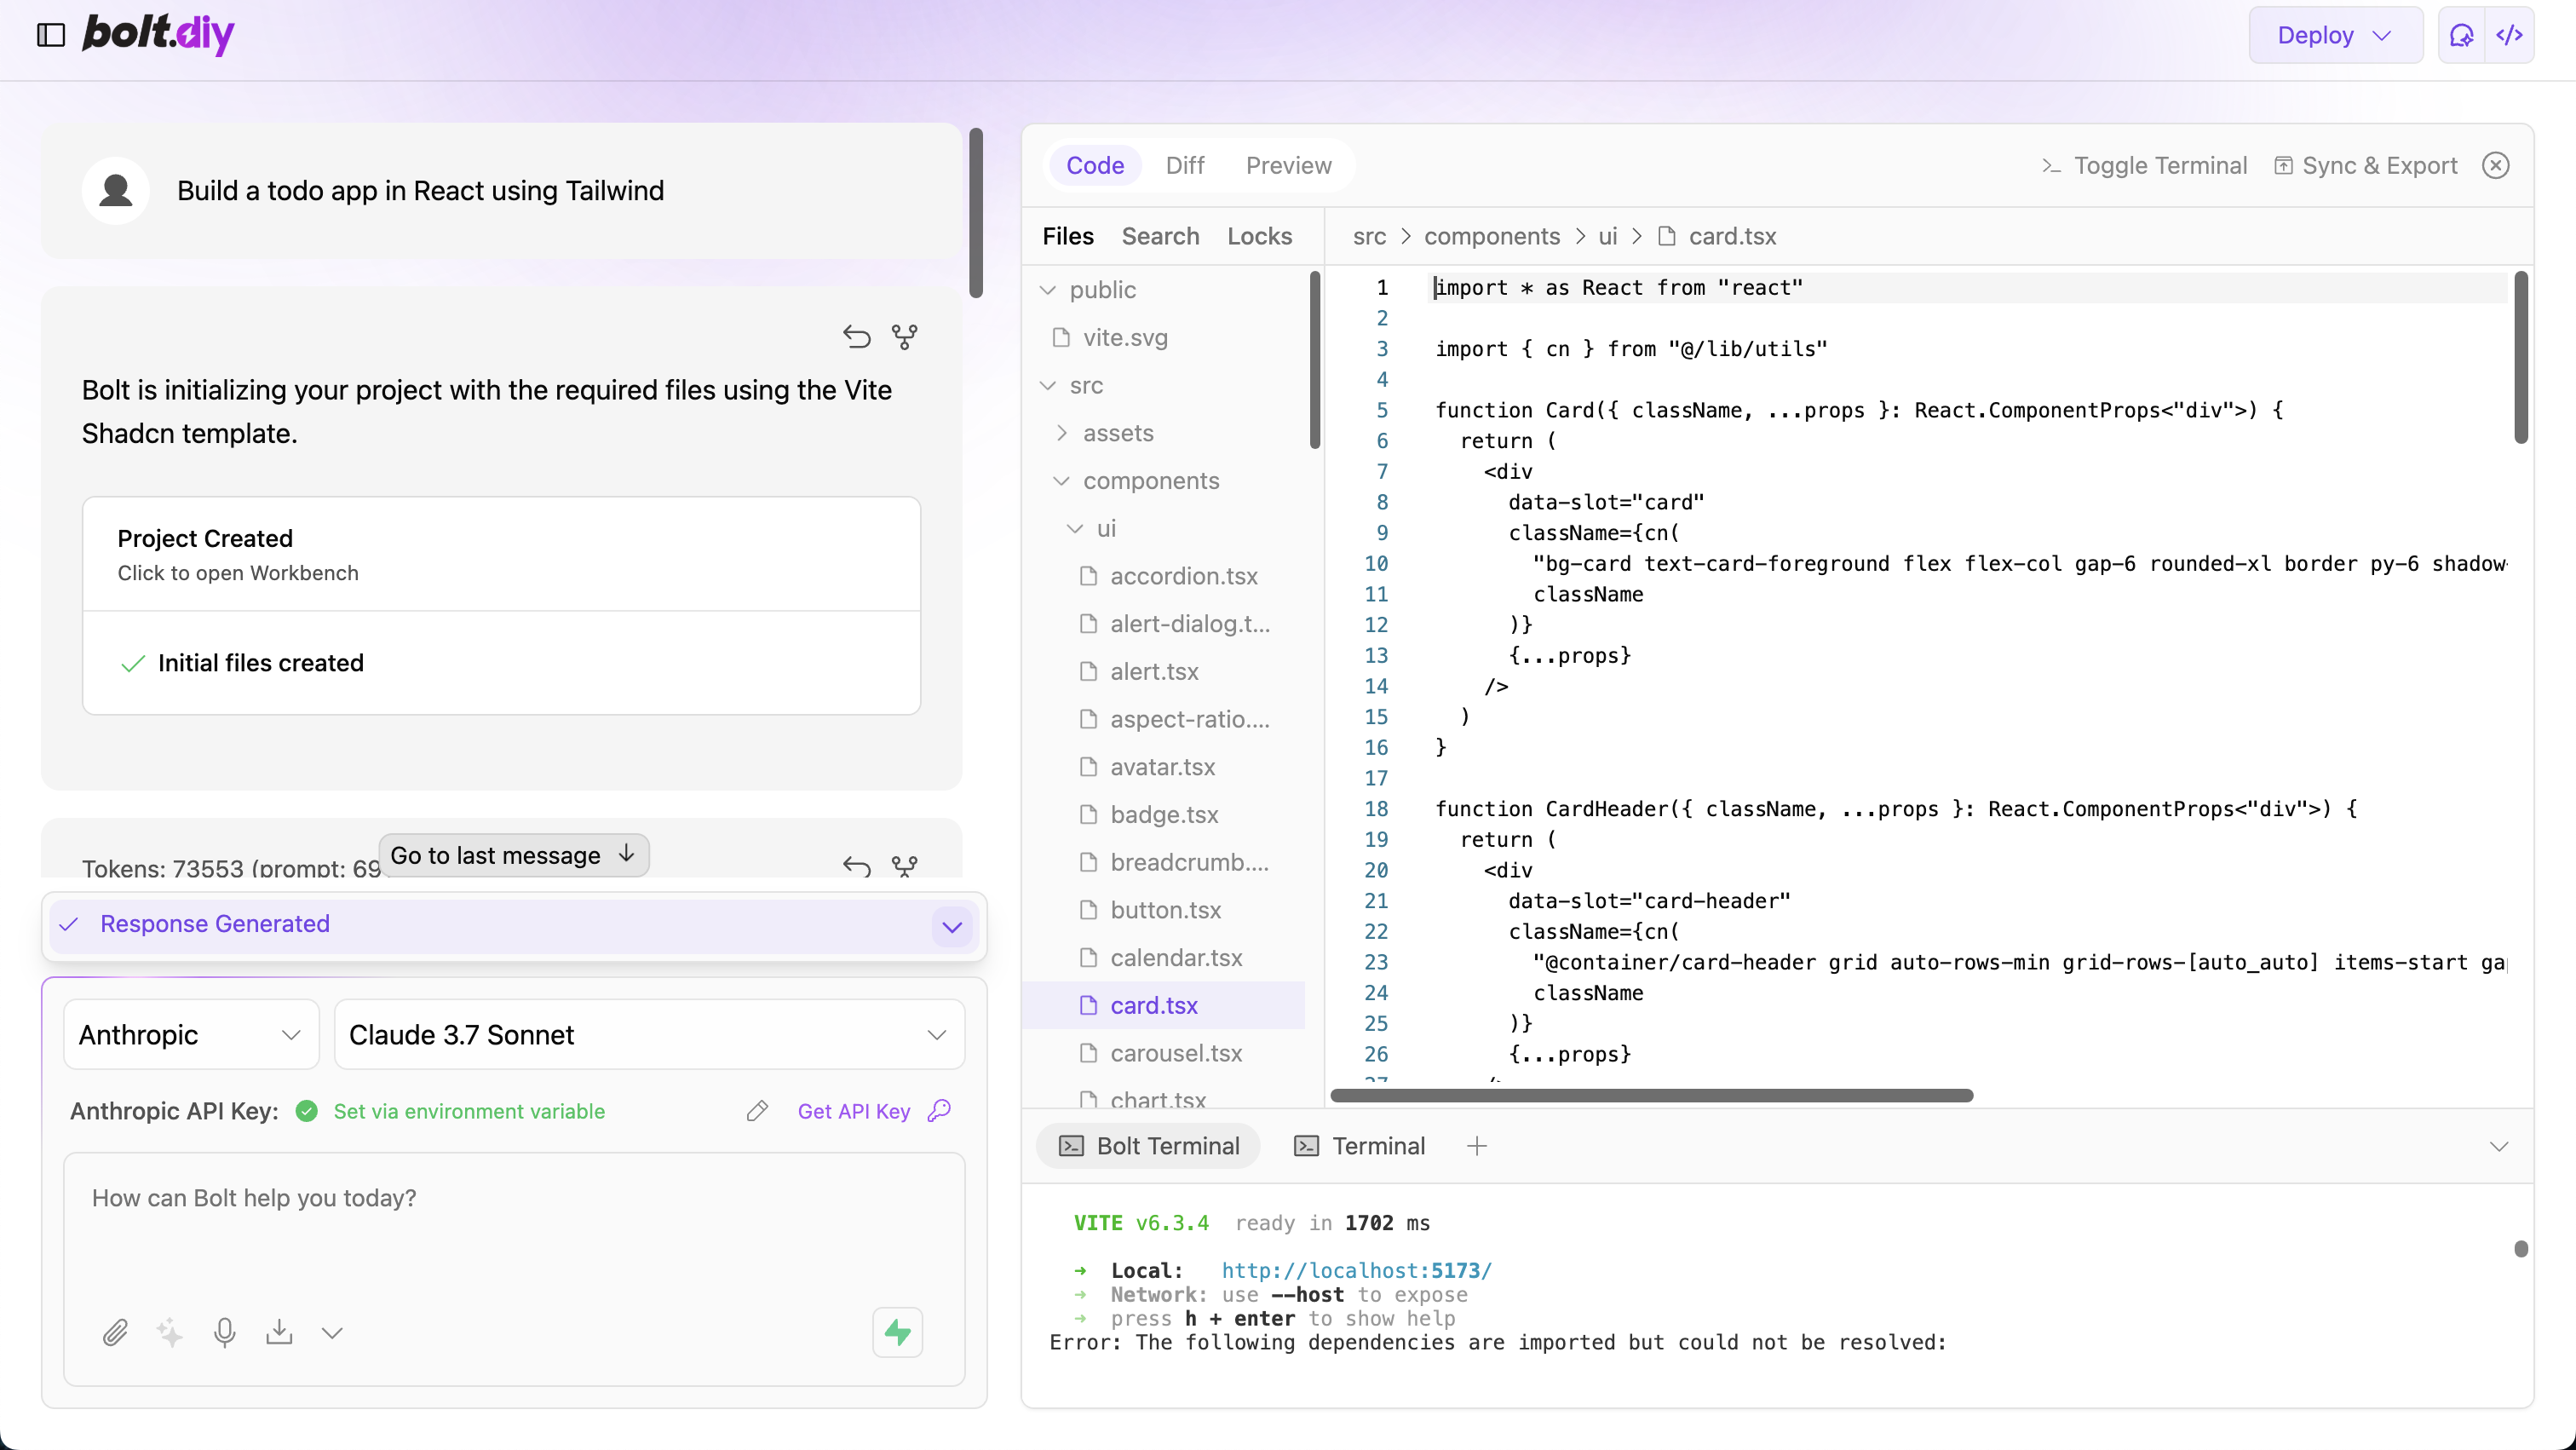
\includegraphics[width=\textwidth]{figures/bolt-diy-example.png}
  \caption{bolt.diy用户界面示例}
  \label{fig:bolt_diy_example}
\end{figure}

\subsection{MessageParser}

MessageParser是bolt.diy的核心组件,负责解析LLM生成的XML格式输出。LLM会生成结构化的XML响应,而MessageParser则识别和提取这些XML中的代码内容、文件路径、执行命令等元信息。

以下示例展示了一个典型的LLM生成的XML结构,描述创建JavaScript阶乘函数的完整过程:

\begin{minted}{xml}
<example>
  <user_query>
    Create a JS function to compute factorial.
  </user_query>
  <assistant_response>
    Certainly, Let's create a factorial function.
    <boltArtifact id="factorial-function" 
                  title="JavaScript Factorial Function">
      <boltAction type="file" filePath="index.js">
        function factorial(n) {
          return n <= 1 ? 1 : n * factorial(n - 1);
        }
      </boltAction>

      <boltAction type="shell">
        node index.js
      </boltAction>
    </boltArtifact>
  </assistant_response>
</example>
\end{minted}

在这个XML结构中,主要包含以下几个标签:

\begin{itemize}
    \item \textless user\_query\textgreater:包含用户的原始自然语言请求,本例中为创建计算阶乘的JavaScript函数。
    \item \textless assistant\_response\textgreater:包含LLM的完整响应,包括文本回复和后续操作步骤,通常通过嵌套的`boltArtifact`和`boltAction`标签表示。
    \item \textless boltArtifact\textgreater:作为容器标签,表示一个完整的代码生成单元或"工件",具有唯一标识符和描述性标题。
    \item \textless boltAction\textgreater:表示具体操作步骤,根据type属性的不同可执行不同类型的操作,例如:
    \begin{itemize}
        \item type="file":创建或修改文件,其中filePath属性指定目标文件路径,标签内容为文件内容。
        \item type="shell":执行命令行操作,标签内容为需执行的shell命令。
    \end{itemize}
\end{itemize}

MessageParser在运行过程中解析LLM输出的文本内容,识别其中的结构化信息。每个操作步骤被封装为`boltAction`,相关操作组合为`boltArtifact`,最终形成完整的代码生成工作流。系统随后根据解析结果,通过FileStore存储生成的代码文件,并由ActionRunner执行相应的命令,实现从自然语言到可执行代码的转换过程。

\subsection{WebContainer技术}

WebContainer是bolt.diy的核心技术之一,由StackBlitz开发的基于WebAssembly的微型操作系统。它通过将Node.js编译为WebAssembly,实现了在浏览器中原生运行Node.js环境的能力。

在技术实现上,WebContainer利用WebAssembly技术在浏览器中模拟完整的操作系统环境,包括文件系统和进程管理等功能。这使开发者能够在浏览器中执行各种命令,如\texttt{npm install}、\texttt{node index.js}等,实现完整的开发工作流程。

在bolt.diy中,WebContainer主要用于提供安全、隔离的代码运行环境。生成的代码通过FileStore存储在WebContainer的虚拟文件系统中,并由ActionRunner在该环境中执行。执行结果随后返回给用户,形成完整的代码生成-执行-反馈循环。

\section{bolt.SE的技术创新与改进}

基于bolt.diy的原有架构,bolt.SE引入了多项技术改进,重点强化了系统在现代软件工程实践中的适应性。

如图~\ref{fig:bolt_sequence}蓝色部分所示,bolt.SE基于此核心流程,增加了四个关键模块:测试驱动开发(TDD)模块负责测试用例管理与执行;API优先开发模块处理API定义与集成;模型上下文协议(MCP)模块提供外部工具调用能力。

\subsection{API优先开发模块}
API优先(API-First)是现代软件开发中的重要方法,强调在实现具体功能前先设计和定义API接口。bolt.SE在此方面的创新体现为构建了基于OpenAPI规范的API定义与管理系统。

该模块允许用户通过界面定义API规范,系统随后将这些规范转化为LLM可理解的结构化指导信息。基于这些信息,LLM能够生成符合预定义API规范的代码实现,确保生成代码与系统整体架构的一致性。

在具体实现上,bolt.SE开发了全新的APIActions组件,包括:
\begin{itemize}
  \item \texttt{ApiActionsContextTags}:显示聊天界面中选中的API标签
  \item \texttt{ApiActionsModal}:管理API的主要模态窗口
  \item \texttt{EditApiActionsModal}:创建和编辑API的编辑器界面
\end{itemize}

这些组件与bolt.diy的文件存储和对话管理系统整合,扩展了原有框架的功能边界。例如,APIActions模块在用户选择API时,将API描述信息压缩,仅保留端点信息与参数定义的核心要素,相比原始描述节省token消耗,优化了bolt.diy的上下文管理机制。

\subsection{测试驱动开发(TDD)模块}

测试驱动开发是一种强调"测试先行"的软件开发方法。bolt.SE通过构建TDD模块,将这一理念与LLM代码生成相结合,形成了一套完整的测试驱动型代码生成流程。

TDD模块与bolt.diy的WebContainer集成,利用其JavaScript执行能力,实现了测试用例的实时运行与验证。当测试失败时,系统自动将错误信息回传给LLM,引导其进行针对性修复,形成完整的"红-绿-重构"循环。

在bolt.diy的设计中,代码生成主要依赖自然语言描述,缺乏结构化的验证机制。bolt.SE的TDD模块在此基础上引入了基于Jest的测试框架集成,实现了测试用例的创建、管理与执行,提升了生成代码的可靠性与质量。

\subsection{模型上下文协议(MCP)模块}

bolt.SE引入了模型上下文协议(Model Context Protocol, MCP),实现LLM与外部工具和数据源的交互。该协议定义了一套标准化接口,使LLM能够安全地调用外部功能。

在技术实现上,MCP模块采用模块化架构设计,支持多种传输方式(如stdio、HTTP SSE)和服务类型。这种灵活性使系统能够适应从本地文件访问到远程服务调用的广泛场景,增强了LLM的功能边界。

bolt.diy原有架构中,LLM主要通过生成XML结构化指令调用系统内置功能,如文件创建和命令执行。bolt.SE的MCP模块扩展了这一机制,实现了与外部工具和服务的标准化集成。MCP为每个外部工具定义了JSON Schema描述,使LLM能够理解工具功能并正确构造调用参数。

